\documentclass{exam}
\usepackage[utf8]{inputenc}
\usepackage[margin=1in]{geometry}
\usepackage{amsmath}
\usepackage{siunitx}
\usepackage{graphicx}
\usepackage{multicol}
\newcommand{\hidepoints}{\pointsinmargin\pointformat{}}
\newcommand{\showpoints}{\nopointsinmargin\pointformat{(\thepoints)}}

\usepackage{xcolor}
\newcommand{\choiceblank}[1]{
	\ifprintanswers \underline{\ \ #1\ \ }
	\else \underline{\hspace{0.40 in}}
	\fi
	\vspace{0.05 in}
}
\newcommand{\fixcolspacing}{\vspace{0pt plus 1filll}\mbox{}}
\renewcommand{\solutiontitle}{}
\unframedsolutions
\SolutionEmphasis{\color{violet}}
\usepackage{etoolbox}
\usepackage{intcalc}
\usepackage{framed}
\usepackage{tabu}
\usepackage{tabularx}
\newcommand{\match}[2]{
	\begin{tabularx}{\textwidth}{r X}
		\fillin[#1][0.5 in] & #2
	\end{tabularx}}
\newcounter{wbcount}
\newcommand{\wbelem}[1]{\stepcounter{wbcount}
	\textbf{\Alph{wbcount}} & {#1}
	\ifnumequal{0}{\intcalcMod{\value{wbcount}}{\wbcolsize}}
		{\\}
		{&}
}
\newenvironment{wordbank}[1]{
	\renewcommand*{\arraystretch}{1.5} \def\wbcolsize{#1}
	\begin{center} \begin{framed}
	\begin{tabu} to \textwidth {*{#1}{X[1,l] X[5,l]}}
	}
	{\end{tabu} \end{framed} \end{center}
}
\setlength\answerclearance{3 pt}


\pagestyle{head}
\header{Class}{Exam title - Page \thepage}{Student ID:\kern .5 in}
\headrule

\begin{document}
\begin{coverpages}
		\vspace{0.00 in}
		\vspace{0.00 in}
	\begin{center}
		\vspace{0.05 in}
		\par\noindent\textbf{\large  Subtitle}
		\vspace{0.05 in}
		\vspace{0.10 in}
		\par\noindent\textbf{\Huge   Title}
		\vspace{0.5 in}
		\vspace{0.05 in}
		\par\noindent
				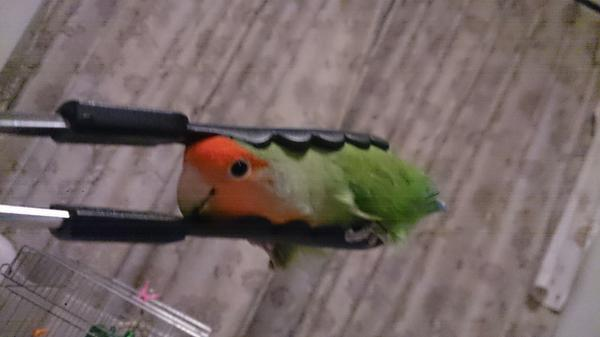
\includegraphics[width=.7\textwidth]{images/tong.jpg}
		\vspace{0.05 in}
		\vspace{0.5 in}
		\vspace{0.10 in}
		\vspace{0.15 in}
		\def\arraystretch{2}\tabcolsep=3pt
		\begin{tabular}{l r}
			\textbf{Student Name:} & \makebox[4in]{\hrulefill} \\
			\textbf{Date:} & \makebox[4in]{\hrulefill} \\
			\textbf{Any other info:} & \makebox[4in]{\hrulefill} \\
		\end{tabular}
		\vspace{0.15 in}
	\end{center}
		\vspace{0.15 in}
	\par The order of modules within sections roughly corresponds to the order in which they're generated as tex. For example, putting the subtitle module before the title module results in the subtitle being rendered above.
	\par Throughout the exam, you can use the following bangs: gap (which inserts vertical space), img (which inserts an image with the given filename and renders it at the given width), options (where you can toggle certain formatting options), and newpage (self explanatory).
		\vspace{0.15 in}
	\begin{center}
		\vspace{0.05 in}
		\par\noindent\textbf{Written by:  Dhruva Karkada}, \textit{ dkarkada@gmail.com}
		\vspace{0.05 in}
	\end{center}
\end{coverpages}

\newpage
\par\noindent \textbf{\large  Part I: Matching}
\par\noindent  2 points each. Each choice will be used; some more than once.
\begin{wordbank}{3}
	\wbelem{Answer 1}
	\wbelem{Answer 2}
	\wbelem{Answer 3}
	\wbelem{Answer 4}
	\wbelem{Answer 5}
	\wbelem{Answer 6}
	\wbelem{Answers}
	\wbelem{Otherwise}
	\wbelem{Questions}
	\wbelem{The option}
	\wbelem{Unless}
\end{wordbank}
\begin{questions}
\setcounter{question}{0}
	\hidepoints
	\question\match{G}{ which are used more than once will only appear once in the wordbox}
	\question\match{J}{ ans=sheet will create a separate answer sheet at the end}
	\question\match{B}{ This is question 2}
	\question\match{K}{ You include 'noshuffle' as an option}
	\question\match{C}{ This is question 3}
	\question\match{F}{ This is question 6}
	\question\match{I}{ Will automatically shuffle}
	\question\match{G}{ are sorted alphabetically, while}
	\question\match{D}{ This is question 4}
	\question\match{E}{ This is question 5}
	\question\match{H}{ No dedicated answer sheet will be created}
	\question\match{A}{ This is question 1}
	\showpoints
\end{questions}

\newpage
\par\noindent \textbf{\large  Part II: Multiple Choice}
\par\noindent  2 points each.
\setlength{\columnsep}{0.40 in}
\begin{multicols*}{2}
\renewcommand{\choiceshook}{\setlength{\leftmargin}{0.40 in}}
\renewcommand{\questionshook}{\setlength{\leftmargin}{0.0 in}}
\begin{questions}
\setcounter{question}{12}
	\question New sections autmatically
	\begin{choices}
		\choice z
		\CorrectChoice Create a pagebreak
		\choice z
	\end{choices}
	\question Multiple choice questions
	\begin{choices}
		\choice z
		\CorrectChoice automatically have answers shuffled
		\choice z
		\choice z
	\end{choices}
	\question Unless you mark the correct answer
	\begin{choices}
		\CorrectChoice with this symbol at the end:
		\choice 1
		\choice 2
		\choice 3
	\end{choices}
	\question Then the answer choice order for that question
	\begin{choices}
		\choice will
		\choice be
		\CorrectChoice preserved
	\end{choices}
	\question The spacing of MC questions depends
	\begin{choices}
		\choice on the available space on the page
		\CorrectChoice which depends on how much instructions you wrote.
	\end{choices}
	\question So do me a favor and estimate the height taken up by the
	\begin{choices}
		\choice title and instructions
		\CorrectChoice measured in units of pt
		\choice and include that as the option ``intro-height''
		\choice z
		\choice z
		\choice z
	\end{choices}
	\question Better to overestimate than underestimate
	\begin{choices}
		\choice z
		\choice z
		\CorrectChoice or else you might get some funky formatting
	\end{choices}
	\vfill\null\columnbreak
	\question The option ``twocolumn'' does what you think it does
	\begin{choices}
		\CorrectChoice z
		\CorrectChoice z
		\CorrectChoice z
	\end{choices}
\end{questions}
\end{multicols*}
\renewcommand{\choiceshook}{}
\renewcommand{\questionshook}{}

\newpage
\par\noindent \textbf{\large  Part III: Free Response}
\par\noindent  Write legibly
\begin{questions}
\setcounter{question}{20}
\question A question can have parts and subparts
	\begin{parts}
	\part Here is a part
		\begin{solution}[20 pt]
		Here is its solution
		\end{solution}
	\part Here is another part
		\begin{subparts}
		\subpart Its first subpart
			\begin{solution}[20 pt]
			and respective solution
			\end{solution}
		\subpart Next subpart
			\begin{solution}[20 pt]
			and respective solution
			\end{solution}
		\end{subparts}
	\part Last part
		\begin{solution}[20 pt]
		solution
		\end{solution}
	\end{parts}
\question You can put math here: $y=mx+b$ or alternatively \[i\hbar \frac{\partial \Psi}{\partial t} = -\frac{\hbar^2}{2m}\frac{\partial^2 \Psi}{\partial x^2} + V \Psi\] if you like this better.
	\begin{solution}[20 pt]
	solution can have $math$ as well
	\end{solution}
\question Quotation ``marks'' and \% symbols are preserved
	\begin{solution}[20 pt]
	solution
	\end{solution}
\question[3]  Indicate point values by preceding questions with curly bracketed numbers
	\begin{parts}
	\part question1
		\begin{solution}[20 pt]
		 And the number of lines the solution will take up
		\end{solution}
	\part question2
		\begin{solution}[100 pt]
		If solution size is not explicitly given, it'll try to guess based on the solution you've written. If you write a really long solution, then it will try to allocate more space for the student to match. But sometimes you want to write a long, detailed solution even though the expected solution may not be as long, so it's better to specify the expected number of lines.
		\end{solution}
	\end{parts}
\question You can also directly put some \LaTeX\ commands in here
	\begin{solution}[20 pt]
	and they \textit{should} work
	\end{solution}
		\newpage
\end{questions}
	\par \section*{Section title}
	\par Lorem ipsum blah blah
	\par \par\noindent Here is some introductory text and stuff
\begin{questions}
\setcounter{question}{25}
\question Back to some sweet
	\begin{parts}
	\part free
		\begin{solution}[20 pt]
		free
		\end{solution}
	\part response
		\begin{solution}[20 pt]
		response
		\end{solution}
	\part questions!
		\begin{solution}[20 pt]
		questions
		\end{solution}
	\end{parts}
\question By default, no answer sheet is generated at the end of the exam. You must use the ans option to specify if you want an answer sheet for a given question module
	\begin{solution}[20 pt]
	ok
	\end{solution}
\question But of course, every question module shows up in the answer key
	\begin{solution}[20 pt]
	of course
	\end{solution}
\end{questions}
\newpage
\section*{Answer Sheet}
\par\noindent \textbf{\large  Part I: Matching}
	\raggedcolumns
	\begin{multicols}{5}
	\begin{enumerate}
	\setcounter{enumi}{0}
	\item \choiceblank{G}
	\item \choiceblank{J}
	\item \choiceblank{B}
	\item \choiceblank{K}
	\item \choiceblank{C}
	\item \choiceblank{F}
	\item \choiceblank{I}
	\item \choiceblank{G}
	\item \choiceblank{D}
	\item \choiceblank{E}
	\item \choiceblank{H}
	\item \choiceblank{A}
	\end{enumerate}
	\fixcolspacing
	\end{multicols}
\par\noindent \textbf{\large  Part II: Multiple Choice}
	\raggedcolumns
	\begin{multicols}{5}
	\begin{enumerate}
	\setcounter{enumi}{12}
	\item \choiceblank{B}
	\item \choiceblank{B}
	\item \choiceblank{A}
	\item \choiceblank{C}
	\item \choiceblank{B}
	\item \choiceblank{B}
	\item \choiceblank{C}
	\item \choiceblank{A}
	\end{enumerate}
	\fixcolspacing
	\end{multicols}
\end{document}